
\begin{figure}
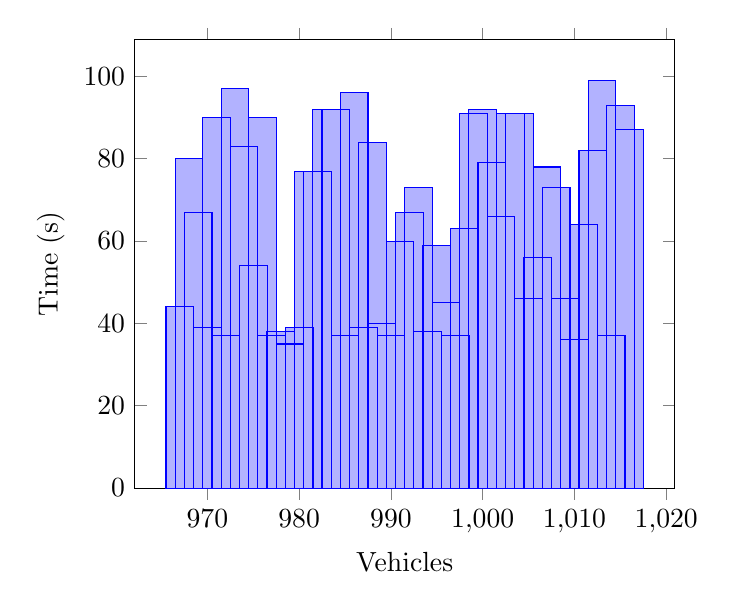
\begin{tikzpicture}
\begin{axis}[
legend style={anchor=west},
xlabel=Vehicles,
ylabel=Time (s),
ymin=0,
ybar,
]
\addplot coordinates {
(1014, 37)
(1015, 93)
(1016, 87)
(1010, 36)
(1012, 82)
(1013, 99)
(1004, 91)
(1002, 66)
(1000, 92)
(1006, 56)
(1009, 46)
(1008, 73)
(1007, 78)
(1005, 46)
(1001, 79)
(977, 37)
(976, 90)
(975, 54)
(974, 83)
(973, 97)
(972, 37)
(971, 90)
(970, 39)
(979, 35)
(978, 38)
(995, 59)
(994, 38)
(997, 37)
(996, 45)
(991, 60)
(990, 37)
(993, 73)
(992, 67)
(999, 91)
(998, 63)
(1011, 64)
(1003, 91)
(967, 44)
(968, 80)
(969, 67)
(987, 39)
(988, 84)
(989, 40)
(982, 77)
(983, 92)
(980, 39)
(981, 77)
(986, 96)
(984, 92)
(985, 37)
};

\end{axis}
\end{tikzpicture}
\label{tik:time:0:90}
\caption{0 percent diving with GSC on route $90$}
\end{figure}
